\chapter{Model Quality and the Bias-Variance Tradeoff \label{chapter:biasvariance}}

We have now seen several different algorithms (and meta-algorithms) for supervised learning. We've examined linear models for classification and regression (Chapters~\ref{chapter:linreg} and \ref{chapter:logreg}), KNN (Chapters~\ref{chapter:classification} and \ref{chapter:regression}), decision trees (Chapters~\ref{chapter:decisiontrees}), and ensemble methods -- usually based on decision trees -- including random forests (Chapter~\ref{chapter:randomforests}) and boosting (Chapter~\ref{chapter:boosting}). In this short chapter, we'll take a step back and talk about some key themes that are relevant to all of these methods. 

%%%%%%%%%%%%%%%%%%%%%%%%%%%%%%%%%%%%%%%%%%%%%%%%%%%%%%%%%%%%%%%%%%%%%%%%%%%%%%%%%

\section{Measuring Error: Loss and Objective Functions}

Most of us think of error as a fairly intuitive concept, and so far in our discussions of model building and model quality, we've avoided any formal definitions. However, as we begin to extend the concepts we've learned from classification and regression to more challenging problem classes (e.g., survival analysis), a more formal conception of what error means and how to minimize it algorithmically becomes increasingly crucial. Here are some examples:

\begin{itemize}
\item In classification, error typically means either the total number of misclassified points,
$$ \text{error} = \sum_{i=1}^n \mathcal{I}\left(y^{(i)} \neq \hat{y}^{(i)}\right), $$
or a weighted average of the number of misclassified points per class. Another way of quantifying classification error is \textbf{AUC}, the area under the receiver operating characteristic curve, which is the probability that a randomly chosen positive example (where $y=1$) will receive a higher score from the model (higher $\hat{y}$) than a randomly chosen negative example (where $y=0$). 
\item In regression, error typically means the \textbf{mean-squared error (MSE)},
$$ \text{error} = \frac{1}{n} \sum_{i=1}^n \left( y^{(i)} - \hat{y}^{(i)} \right)^2, $$
although there are also other ways of quantifying error. For example, you could use the \textbf{mean absolute error}
$$ \text{error} = \frac{1}{n} \sum_{i=1}^n \vert y^{(i)} - \hat{y}^{(i)} \vert. $$
Neither is ``wrong'' or ``right'', but they have different properties. For example, the MSE gives a higher weight to large errors (outliers). It's also differentiable, which is why it's used so much more often in, e.g., neural networks than the mean absolute error. 
\item In survival analysis, error is typically quantified using something called \textbf{Harrell's concordance index}, which takes into account censored observations\footnote{For a detailed explanation and some experimental results, see Kattan MW, Hess KR and Beck JR (1998). ``Experiments to determine whether recursive partitioning (CART) or an artificial neural network overcomes theoretical limitations of Cox proportional hazards regression.'' \emph{Computers and Biomedical Research}, 31(5), 363-373.}.
\end{itemize}

\vspace{2mm}

\begin{question}{question:harrell}
Harrell's concordance ($C$) index is probably unfamiliar to you. It is calculated like this:
\begin{enumerate}
\item Create a list of all possible pairs of patients. There will be $n(n-1)/2$ pairs.
\item Eliminate all pairs for which the patient with the shorter follow-up time does not experience the event of interest (i.e., is censored). The remaining patient pairs are considered ``usable'' since the patient with the shorter time-to-event is identifiable. 
\item Count the number of usable patient pairs for which the patient with the shorter follow-up time had the higher predicted hazard for the event. That is, you want the number of pairs for which the model's predictions about relative times to event are consistent with the observed data.
\item The $C$ statistic is the number of consistent pairs divided by the number of usable pairs. The error is defined as $1-C$. 
\end{enumerate}
Here are four patients and the predicted mean time to event from two different survival models (low value means lower time to event). All times are in years. Calculate the $C$ statistic for both models.

    \begin{center}
    \begin{tabular}{ccccc}
    \toprule
    Patient & Follow-up Time & Observed? & Model 1 Score & Model 2 Score \\
    \midrule
    1 & 8.3 & 1 & 4.6 & 5.2 \\
    2 & 6.5 & 0 & 2.3 & 7.1 \\
    3 & 2.7 & 1 & 0.6 & 6.7 \\
    4 & 7.4 & 1 & 4.7 & 6.6 \\
    \bottomrule
    \end{tabular}
    \end{center}
    
{\small
    \begin{center}
    \begin{tabular}{ccccc}
    \toprule
    First Patient & Second Patient & Usable & Model 1 & Model 2 \\
    & & & Consistent & Consistent \\
    \midrule
    1 & 2 & \\
    1 & 3 & \\
    1 & 4 & \\
    2 & 3 & \\
    2 & 4 & \\
    3 & 4 & \\
    \bottomrule
    \end{tabular}
    \end{center}
}
You should find that the $C$ statistic for Model 1 is 0.75, while the $C$ statistic for Model 2 is only 0.25. Model 1 is clearly the better model.
\end{question}

The definition of error used to optimize a particular model is called a \textbf{loss function}. Loss functions are a general concept from optimization and decision theory; they represent the cost associated with a decision. If we think of a supervised learning model as an engine for making decisions, the loss is how ``bad'', on average, those decisions will be. Loss functions are, in turn, part of a broader class of functions called \textbf{objective functions}. Most learning algorithms work by either minimizing some measure of ``badness'' (a loss function) or maximizing some measure of ``goodness'' (negative of the loss, alternatively called a \textbf{reward function}).
\vspace{2mm}
\begin{question}{}
Imagine what would happen if, in Question~\ref{question:harrell}, we simply set a follow-up time of $7$ years and treated the problem as a classification problem, calculating the AUC for the two models based on that time horizon and ignoring censoring.
    \begin{center}
    \begin{tabular}{ccccc}
    \toprule
    Positive Patient & Negative Patient & Model 1 & Model 2 \\
    & & Ranks Pos Higher? & Ranks Pos Higher? \\
    \midrule
    3 & 1 & 1 & 0 \\
    3 & 2 & 1 & 1 \\
    3 & 4 & 1 & 1 \\
    \bottomrule
    \end{tabular}
    \end{center}
We would calculate an AUC of 1.0 for Model 1 and 0.67 for Model 2. Do you think this is a good approach to quantifying error for this problem? Why or why not?
\end{question}

The choice of how to define error, and which loss function to use for quantifying that error, ultimately rests with the model builder. The process of model training is about adjusting the available parameters of the model to minimize the loss. 

%%%%%%%%%%%%%%%%%%%%%%%%%%%%%%%%%%%%%%%%%%%%%%%%%%%%%%%%%%%%%%%%%%%%%%%%%%%%%%%%%

\section{Goodness of Fit vs. Generalizability}

Once we have an appropriate objective function, we can set about building a model to optimize it. This requires us to think about what constitutes a ``good model''. It's a bit more complicated than simply minimizing the loss on our training data, because ideally we want a model that is both accurate and \textbf{parsimonious}, meaning that it is as simple as possible without sacrificing performance. Another way of thinking about this is that we create models to tell stories about the data we see. If they are good stories, they will do two things:
\begin{enumerate}
\item Explain the structure of the data that are used to train them (high \textbf{goodness of fit})
\item Make accurate predictions on new data (good \textbf{generalizability}) 
\end{enumerate}
For a supervised learning model, we quantify (1) using the \textbf{training error} (error on the training set) and (2) using the \textbf{test error} (error on an independent test set).

\vspace{2mm}

\begin{question}{}
Here we see three decision boundaries for KNN with different values of $K$ (the number of neighbors considered in making a prediction). The data are for the two-class classification problem first discussed in Chapter~\ref{chapter:classification}. From left to right, $K=50, 15,$ and $3$. What are the tradeoffs in moving from left to right in terms of (a) training error/goodness of fit and (b) test error/generalizability? 
\begin{center}
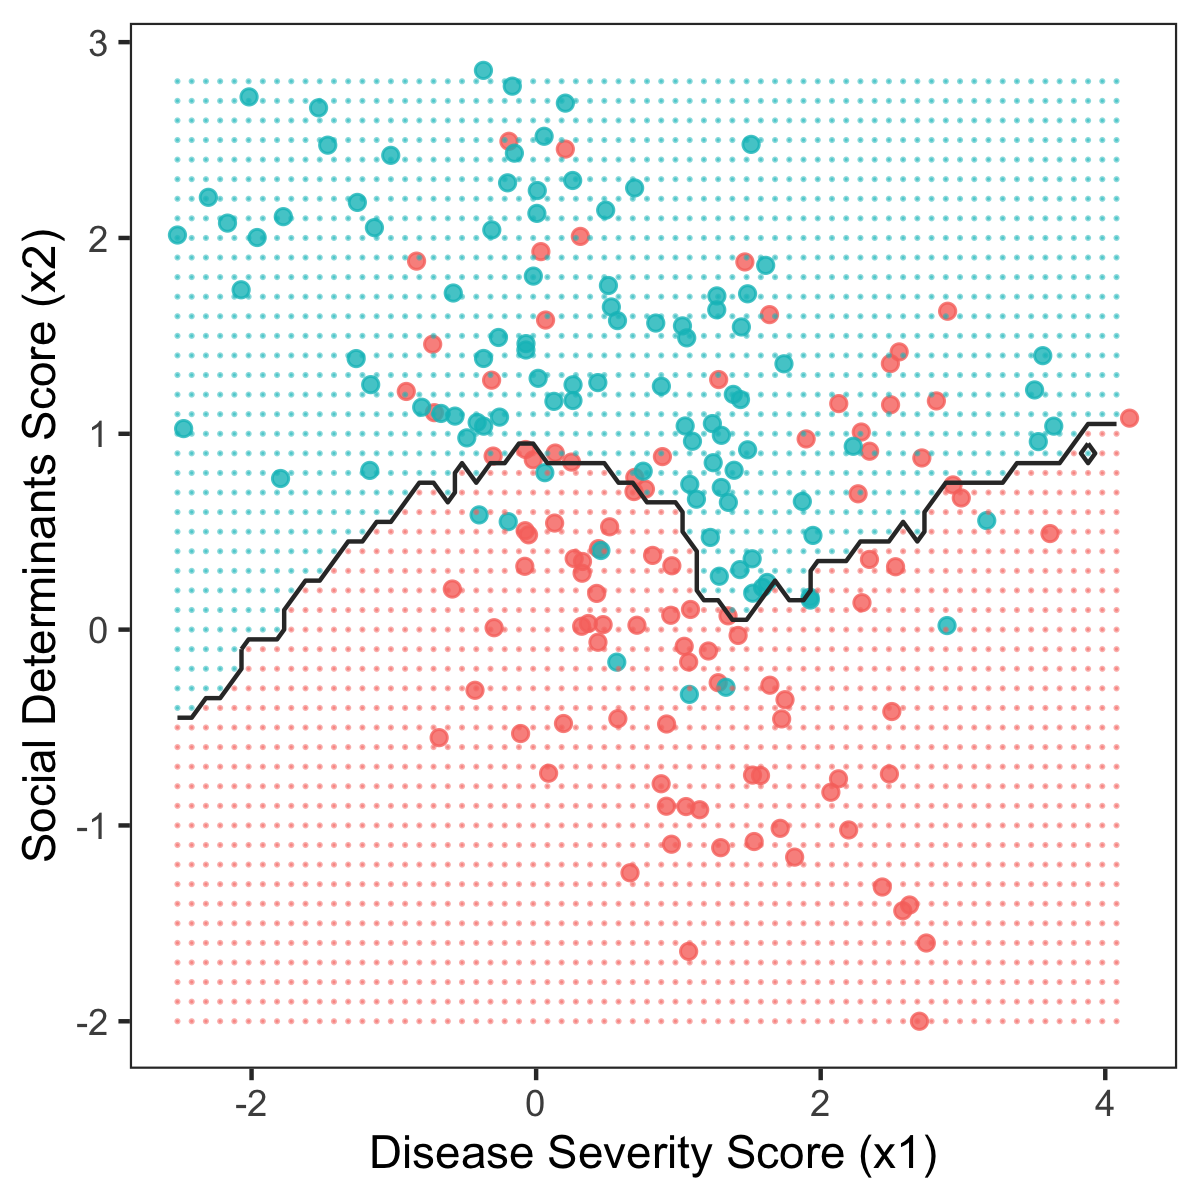
\includegraphics[width=0.3\textwidth]{img/esl-knn-50.png}
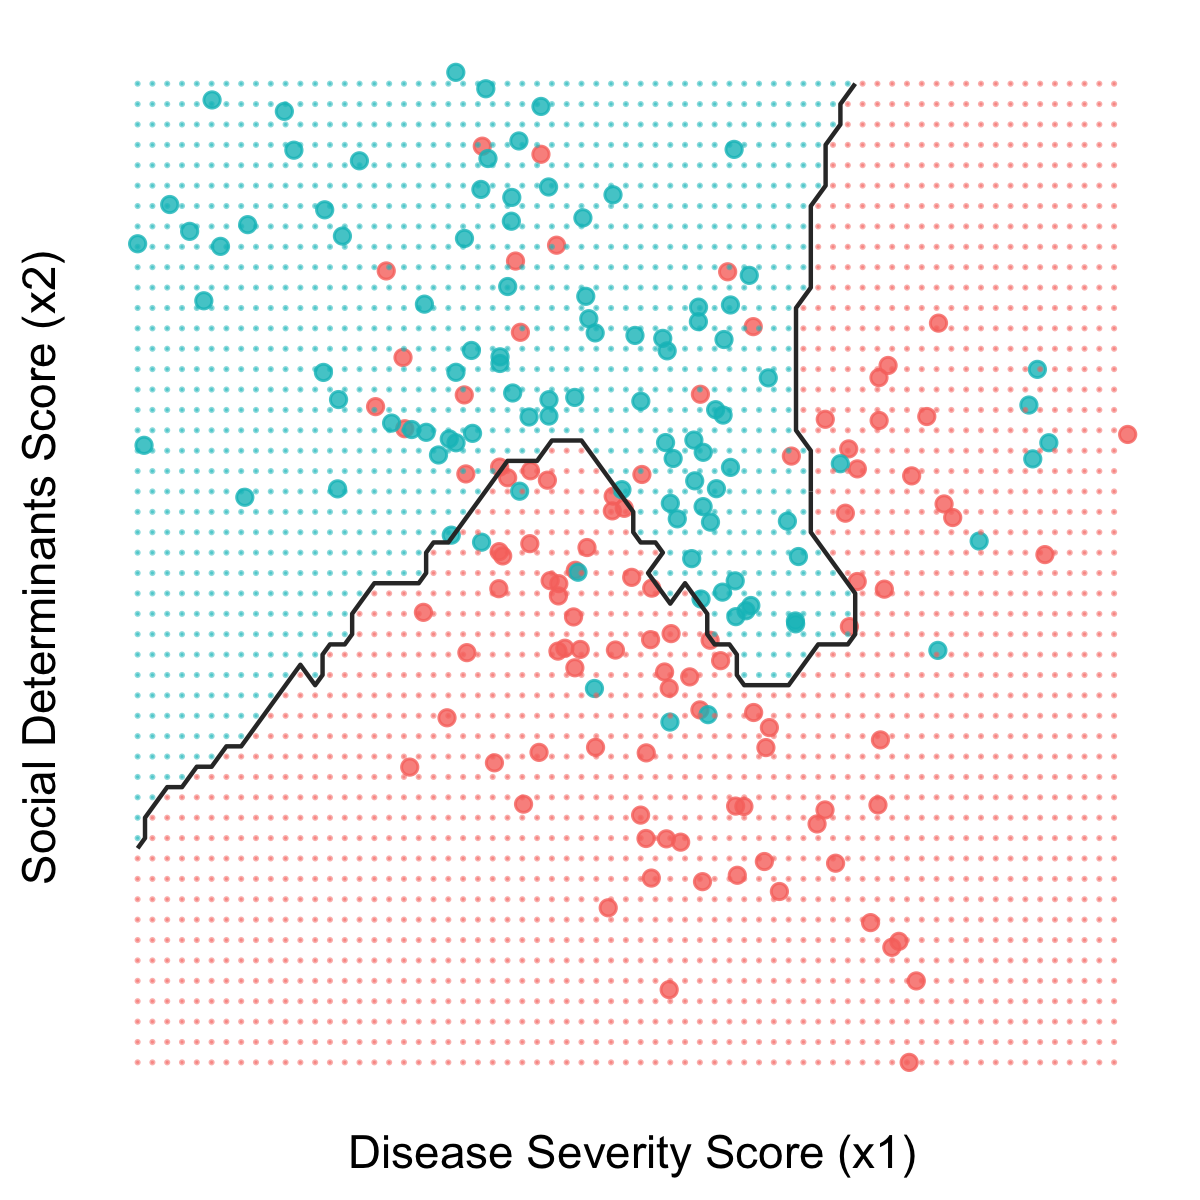
\includegraphics[width=0.3\textwidth]{img/esl-knn-15.png}
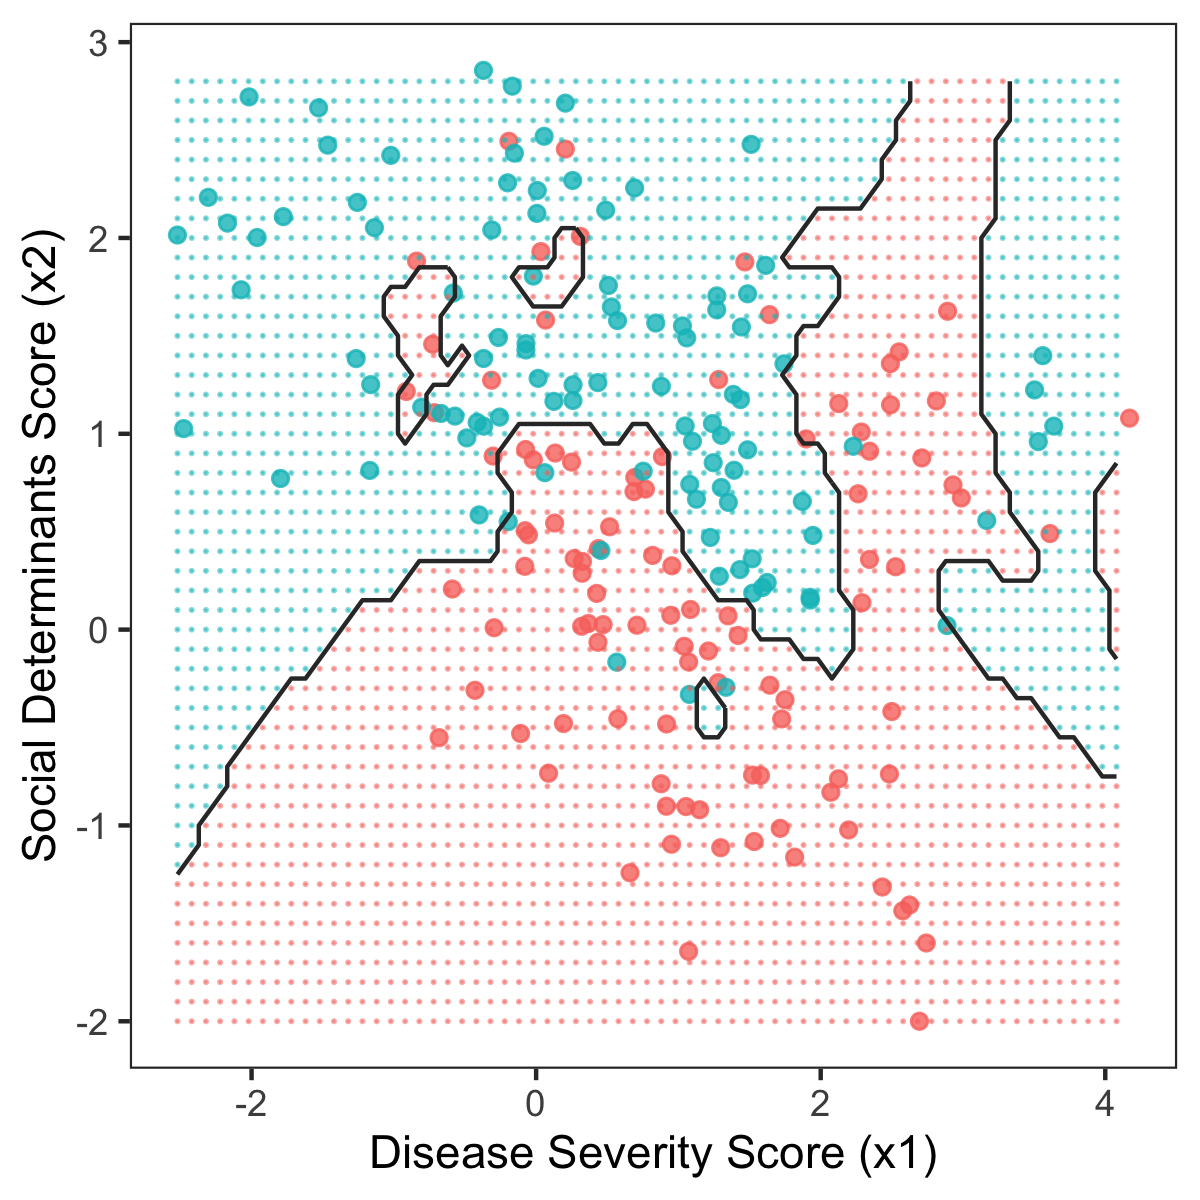
\includegraphics[width=0.3\textwidth]{img/esl-knn-3.png}
\end{center}
\end{question}

In supervised learning, \textbf{model complexity} (loosely defined as the effective number of parameters the model must fit) is, therefore, a very important consideration. A model that is not complex enough will fail to capture all of the structure in the training data, and both its training and test error will suffer as a result. We call this situation \textbf{underfitting}. Conversely, a model that is too complex may fit the training data very well -- maybe perfectly -- but will fail to generalize well to new data. We call this situation \textbf{overfitting}. 

%%%%%%%%%%%%%%%%%%%%%%%%%%%%%%%%%%%%%%%%%%%%%%%%%%%%%%%%%%%%%%%%%%%%%%%%%%%%%%%%%

\section{Bias vs. Variance}

It turns out that there is a general principle governing model complexity in supervised learning called the \textbf{bias-variance tradeoff}. It is perhaps best illustrated by this figure, which comes from the excellent (and free) book \emph{Elements of Statistical Learning}, by Tibshirani, Hastie, and Friedman (Figure 2.11):

\begin{center}
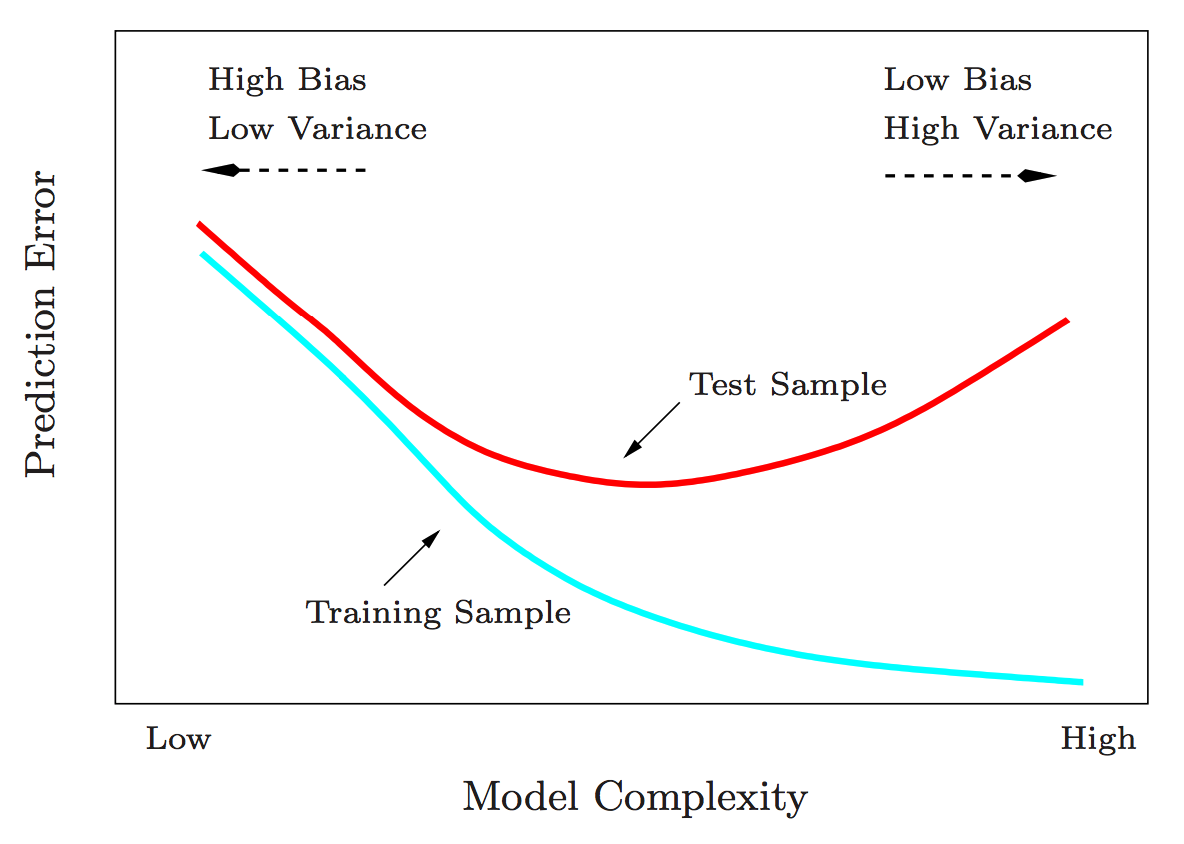
\includegraphics[width=0.8\textwidth]{img/l03-bias-variance-tradeoff.png}
\end{center}

The figure shows us that test error, our measurement of generalization error, comes from two different sources:
$$ \text{test error} = \text{bias} + \text{variance}. $$
The term \textbf{bias} refers to error that results from underfitting, while \textbf{variance} results from overfitting. 

Error due to bias can often be reduced by introducing more/different features or by using a different learning algorithm. Error due to variance can often be reduced by increasing the size or diversity of the training data. That's why it's important to know which situation you're in; gathering more training data when your model is too simple is unlikely to help you, and deploying an extremely fancy (and complicated) deep learning model when logistic regression has already overfit your training data is also unlikely to help. 

Another consideration is that even the ``sweet spot'' (minimum test error) on the bias-variance tradeoff curve can still be high. This occurs when the data you have available simply aren't sufficient to answer the question -- maybe you have the wrong features or there is no relationship between the features and the outcome. Or maybe your features aren't measured correctly. In my experience, these types of issues are not considered often enough in the clinical domain. 

\vspace{2mm}

\begin{question}{}
A recent review article had the provocative title ``A systematic review shows no performance benefit of machine learning over logistic regression for clinical prediction models.'' (Christodoulou E, Ma J, Collins GS, Steyerberg EW, Verbakel JY, Van Calster B. \emph{Journal of Clinical Epidemiology}, 2019, 110:12-22). Assuming this finding is true, what is it telling us about the nature of the error in most clinical risk prediction models? What does it suggest about what we should be doing to improve the performance of these models? 
\end{question}

Another way of thinking about bias and variance is in terms of what happens when you make slight changes to the training data (for example, by collecting new data from the same patient population, or drawing repeated bootstrap samples from the same training set). The figure below is from the article \emph{Understanding the Bias-Variance Tradeoff}, by Scott Fortmann-Roe:

\begin{center}
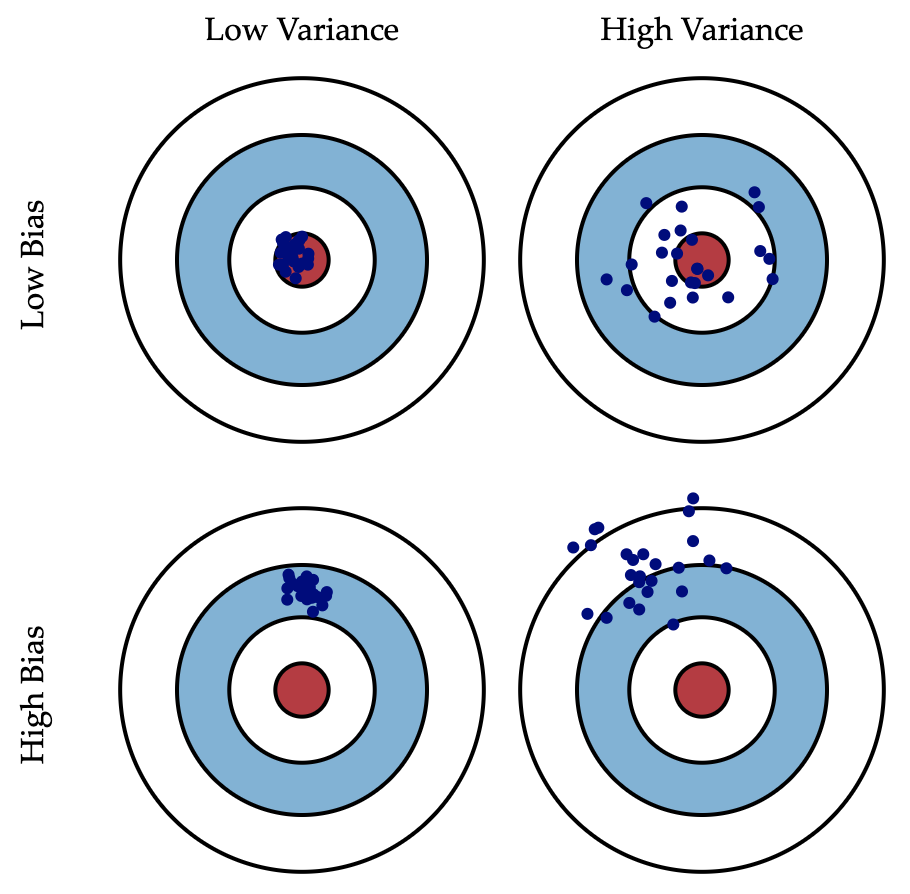
\includegraphics[width=0.7\textwidth]{img/targets-bias-variance.png}
\end{center}

Think of each dot as representing a single test example evaluated under the same model trained on slightly different datasets. The center of the target is the prediction the model should make for that test example. In the case of high bias and low variance, all of the models are off, but they are ``wrong in the same way''. Even if you average their predictions, the answer is still way off the mark. In the case of high variance, the models all make incorrect predictions, but their predictions are off in different directions. As a result, if you average their outputs, you'll get closer to the right answer. 

\vspace{2mm}

\begin{question}{}
We saw random forests in Chapter~\ref{chapter:randomforests} and were introduced to boosting in Chapter~\ref{chapter:boosting}. It is interesting to compare the two methods because they reduce test error in different ways: one primarily tackles variance, while the other primarily tackles bias. Which one is which, and how does each algorithm succeed in reducing its respective form of error? Hint: The image below may help. One column represents three trees from a random forest; the other represents three trees from a boosting model.

\begin{center}
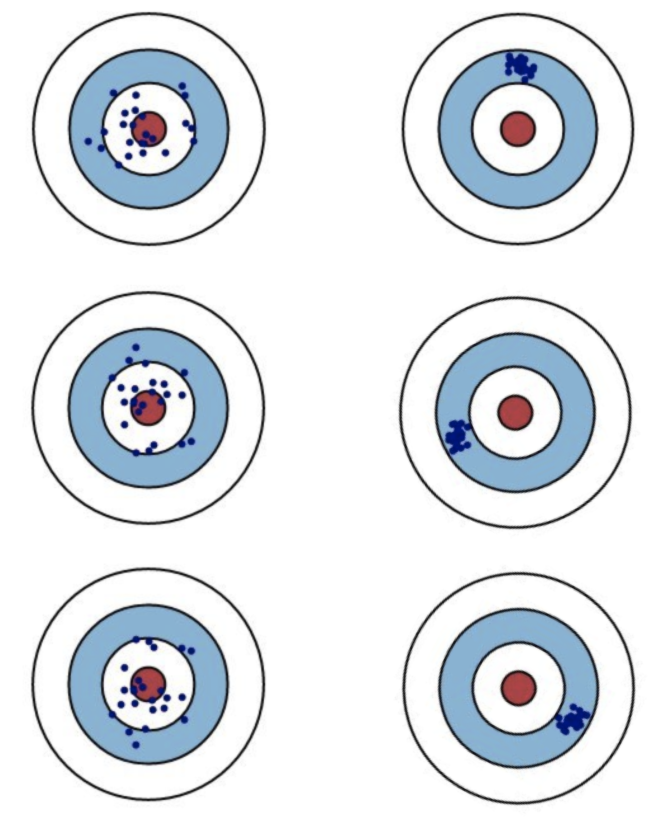
\includegraphics[width=0.7\textwidth]{img/bias-variance-reduction-targets.png}
\end{center}
\end{question}
